\documentclass{amsart}
\usepackage{graphicx,amsfonts,amsthm,amsmath,amssymb,enumerate,enumitem,xcolor,commath,hyperref} % Required for inserting images
\usepackage{geometry}[margin=0.75in]
\usepackage{biblatex}[sorting=none]

\title{An Introduction to Computational Stochastic PDEs\\ Exercises: Chapter 2}
\author{Chris DuPre }
\date{April 2024}

\theoremstyle{plain}
\newtheorem{thm}{Theorem}[section]
\newtheorem{lem}[thm]{Lemma}
\newtheorem{prop}[thm]{Proposition}
\newtheorem*{cor}{Corollary}

\theoremstyle{definition}
\newtheorem{defn}{Definition}[section]
\newtheorem{conj}{Conjecture}[section]
\newtheorem{exmp}{Example}[section]
\newtheorem{exer}{Exercise}[section]

\newcommand{\R}{\mathbb{R}}
\newcommand{\C}{\mathbb{C}}
\newcommand{\Z}{\mathbb{Z}}
\newcommand{\Q}{\mathbb{Q}}
\newcommand{\N}{\mathbb{N}}
\newcommand{\Hil}{\mathcal{H}}
\newcommand{\E}{\mathcal{E}}
\DeclareMathOperator{\csch}{csch}
\DeclareMathOperator{\sech}{sech}

\newcommand{\tcr}[1]{\textcolor{red}{#1}}

\bibliography{Ref}

\begin{document}

\maketitle
\setcounter{section}{2}
\begin{exer}
    Let $V = H_0^1(a,b).$ Show that if Assumption 2.8 in \cite{lord2014introduction} holds, then $a(\cdot,\cdot): V\times V\to \R$ in (2.9) in \cite{lord2014introduction} is an inner product on $V.$
\end{exer}
\begin{proof}
Note that $a$ is clearly symmetric and linear in the first argument. It is also clearly non-negative along the diagonal. Thus, it suffices to show that it is non-degenerate. To see this, note that 
$$a(u,u) ^2= \int_{a}^b p(x) u'(x)^2 dx + \int_a^b q(x) u(x)^2 dx \geq p_0\int_{a}^b u'(x)^2 dx.$$
Thus $a(u,u) = 0$ implies that $\int_a^b u'(x)^2 dx$ which implies $u'(x) = 0$ a.s. As $u \in H_0^1(a,b)$, this implies that $u = 0.$ Thus $a(\cdot,\cdot)$ is a non-degenerate symmetric bilinear form, hence an inner product. 
\end{proof}

\begin{exer}
    Let $p,q$ satisfy the conditions of Assumption 2.8 in \cite{lord2014introduction}. Prove the norm equivalence $(2.14).$ In addition, show that the energy norm $\|\cdot \|_{E}$ is equivalent to the norm $\|\cdot \|_{H^1(a,b)}.$
\end{exer}
\begin{proof}
    To see the upper bounds, not that 
    $$\|u\|_{E}^2 \leq \max\left\{\|p\|_{\infty},\|q\|_{\infty}\right\} \left[\int_a^b u'(x)^2 dx + \int_a^b u(x)^2 dx\right] = \max\left\{\|p\|_{\infty},\|q\|_{\infty}\right\} \|u\|_{H^1(a,b)}^2.$$
    For the lower bound, note that 
    \begin{align*}
        \|u\|_{E}^2 & \geq p_0 \int_a^b u'(x)^2 dx = \frac{p_0}{1+K^2} \int_a^b u'(x)^2 dx + \frac{p_0 }{1+K^2} K^2 \int_a^b u'(x)^2 dx \\
        & \geq \frac{p_0}{1+K^2}\left[\int_a^b u'(x)^2 +u(x)^2 dx \right] = \frac{p_0}{1+K^2} \|u\|_{H^1(a,b)}^2.
    \end{align*}
    Where $K$ is the associated Poincar\'e inequality (take $K = \frac{b-a}{\pi}$). Collecting these gives
    $$\sqrt{\frac{p_0}{1+K^2}}\|u\|_{H^1(a,b)} \leq \|u\|_{E} \leq \max\left\{\sqrt{\|p\|_{\infty}},\sqrt{\|q\|_{\infty}}\right\}\|u\|_{H^1(a,b)}.$$
\end{proof}

\begin{exer}
    Let Assumption 2.8 hold. Assume, for contradiction, that there are two weak solutions $u_1,u_2$ satisfying (2.11) in \cite{lord2014introduction} and show that $u_1 = u_2$. Hence, deduce that (2.11) has at most one solution.
\end{exer}
\begin{proof}
Suppose there exists two solutions $u_1 \neq u_2$ that satisfy (2.11). Then for all $u\in H_0^1(a,b)$
$$a(u,u_1-u_2) = a(u,u_1)-a(u,u_2) = \ell(u)-\ell(u) = 0.$$ 
In particular, this applies for $u = u_1-u_2.$ Thus $\|u_1-u_2\|_{E} = 0.$ By equivalence of norms, $\|u_1-u_2\|_{H_0^1(a,b)} = 0.$ Therefore $u_1 = u_2$, contradiction $\Rightarrow\!\Leftarrow$. 
    
\end{proof}

\begin{exer}
    Let Assumption 2.1 in \cite{lord2014introduction} hold. Consider the operator $A$ given by (2.24) and let $G(x,y)$ denote the Green's function satisfying (2.25).
    \begin{enumerate}[label=\alph*.]
        \item Show that 
        $$G'(x,x_{+}) - G'(x,x_{-}) = \frac{-1}{p(x)},$$
        where $G'(x,x_{+})$ denotes the limit of $G'(x,x+\varepsilon)$ as $\varepsilon$ approaches $0$ from above and $G'(x,x_{-})$ is the limit as $\varepsilon$ approaches $0$ from below. 
        \item Suppose that $u_1,u_2 \in C^{2}([a,b])$ are non-zero functions such that $Au_i = 0$ for $i=1,2$ with $u_1(a)=u_2(b) = 0.$ Show that 
        $$G(x,y) = \begin{cases}
            Cu_1(x)u_2(y) & x\leq y\\
            Cu_2(x)u_1(y) & x>y
    \end{cases}$$
    for a constant that you should determine.
    \item Show that $G(x,y)$ is symmetric and belongs to $L^2\left([a,b]\times[a,b]\right).$
    \end{enumerate}
\end{exer}
\begin{proof}
    \begin{enumerate}[label=\alph*.]
        \item To see this, note that by definition of the Green's function we have that 
        \begin{align*}
            1 &= -\int_{x-\varepsilon}^{x+\varepsilon} \frac{d}{dx}\left(p(x) G'(x,y)\right) + q(x) G(x,y) dx \\
            &= -p(x)\left[\frac{p(x+\varepsilon)}{p(x)}G'(x,x+\varepsilon)- \frac{p(x-\varepsilon)}{p(x)}G'(x,x-\varepsilon) \right] +\int_{x-\varepsilon}^{x+\varepsilon} u(x) G(x,y) dx.
        \end{align*}
        As $p$ is continuous and $G \in H^2$ the fraction terms tend to one and the integral term vanish respectively. Using the continuity of multiplication and the uniform continuity of $p$ over a compact domain gives
        \begin{gather*}
            1 =  -p(x)\left[G'(x,x_{+})- G'(x,x_{-}) \right]\\
            G'(x,x_{+})- G'(x,x_{-}) = \frac{-1}{p(x)}.
        \end{gather*}
        \item As $u_1,u_2$ both satisfy $Au_i = 0$, we claim 
        $p(x)\left[u_1'(x)u_2(x) - u_1(x)u_2'(x)\right]$ is constant.
        Thus in particular 
        $$ u_1(x)u_2'(x)-u_1'(x)u_2(x) = -\frac{p(a)\left[u_1'(a)u_2(a) - u_1(a)u_2'(a)\right]}{p(x)} = -\frac{p(a)u_1'(a)u_2(a)}{p(x)} $$
        To see this, we take the derivative 
        \begin{align*}
            \frac{d}{dx}\left[p(x)\left[u_1'(x)u_2(x) - u_1(x)u_2'(x)\right]\right] &= \frac{d}{dx}\left[p(x)u_1'(x)\right]u_2(x) + p(x)u_1'(x)u_2'(x) \\
            &- p(x)u_1'(x)u_2'(x) - u_1(x)\frac{d}{dx}\left[p(x)u_2'(x)\right]\\
            &= u_1(x)q(x)u_2(x) - u_1(x)q(x)u_2(x) = 0.
        \end{align*}
        We can then compute $G'(x,x_{+})-G'(x,x_{-})$ explicitly 
        $$G'(x,x_{+})-G'(x,x_{-}) = C\left[u_2'(x)u_1(x)-u_1'(x)u_2'(x)\right] = -\frac{Cp(a)u_1'(a)u_2(a)}{p(x)}.$$
        Thus if $C = \frac{1}{p(a)u_1'(a)u_2(a)},$ the jump condition is satisfied. 
        \item As $u_1,u_2$ are in $C^2$, it is clear that the above form is in $L^2([a,b]).$ To show symmetry, note that if $x<y$ we have that 
        $$G(y,x) = Cu_2(y)u_1(x) = G(x,y).$$
    \end{enumerate}
\end{proof}

\begin{exer}
    Fix the coefficients $p=1$ and $q=1.$ Using Algorithms $2.1$ and $2.2$, investigate the condition number of the matrices $A,K$ and $M$ on the finite element mesh width $h$.
\end{exer}
\begin{proof}
    See Problem\_5.ipynb for a more thorough write-up, but roughly the condition number $\kappa$ of $M$ grows like $4-n_e^{-2}$ and the condition number of $K,A$ grow like $n_e^2.$
    \tcr{Include Pictures}
\end{proof}

\begin{exer}
    Using $(2.36)$, show that the local quadratic basis functions associate with the nodes $x_1^k = 0, x_2^k = \frac{h}{2}, x_3^k = h$ on the element $e_k = [0,h]$ are 
    \begin{align*}
        \phi_1^k(x) = \frac{2x^2}{h^2}-\frac{3x}{h}+ 1, && \phi_2^k(x) = \frac{4x}{h}-\frac{4x^2}{h^2}, && \phi_3^k = \frac{2x^2}{h^2}-\frac{x}{h}.
    \end{align*}
    Assume that $q=0$ and $p$ and $f$ are constants. Compute the element vector $\mathbf{b}^k \in \R^3$ and show that the $3\times3$ element matrix $A^k$ for this specific element is 
    $$A^k = \frac{1}{3h}\begin{pmatrix}
        7 & -8 & 1 \\ -8 & 16 & -8\\ 1 & -8 & 7 
    \end{pmatrix}$$
\end{exer}
\begin{proof}
    Note that we seek $\phi_{j}^k(x)$ as a quadratic polynomial such that 
    $$\phi_{j}^k\left(x_l^k\right) = \delta_{jl}.$$
    This immediately allows us to write 
    \begin{align*}
        \phi_1^k(x) &= c_1 \left(x-\frac{h}{2}\right)\left(x-h\right) = c_1\left[x^2 - \frac{3xh}{2} + \frac{h^2}{2}\right]\\
        \phi_2^k(x) &= c_2 x\left(x-h\right)=  c_2\left[x^2 - hx\right]\\
        \phi_3^k(x) &= c_3 x\left(x-\frac{h}{2}\right) = c_3\left[x^2 - \frac{xh}{2}\right].
    \end{align*}
    We can solve for $c_1,c_2,c_3$ as follows
    \begin{gather*}
        \phi_1^k\left(\frac{h}{2}\right) = c_1 \frac{h^2}{2} = 1 \implies c_1 = \frac{2}{h^2}\\
        \phi_2^k\left(\frac{h}{2}\right) = c_2 \left[\frac{h^2}{4}-\frac{h^2}{2}\right] = -c_2 \frac{h^2}{4} = 1 \implies c_2 = \frac{-4}{h^2}\\
        \phi_3^k(h) = c_3 \frac{h^2}{2} = 1 \implies c_3 = \frac{2}{h^2}.
    \end{gather*}
    Plugging these back in give the desired expressions. 
    \par We can then compute $b^k$ by the following three integrals
    \begin{align*}
        \left(b^k\right)_1 &= \int_0^h f \phi_1^k(x) dx = f\int_0^h \frac{2x^2}{h^2}-\frac{3x}{h}+1 dx = f\left[\frac{2x^3}{3h^2}-\frac{3x^2}{2h}+x\right]_{x=0}^{x=h}\\
        &= f \left[\frac{2h}{3}-\frac{3h}{2}+h\right] = \frac{fh}{6}\\
        \left(b^k\right)_2 &= \int_0^h f \phi_2^k(x) dx = f\int_0^h \frac{4x}{h}-\frac{4x^2}{h^2} dx = f\left[\frac{2x^2}{h}-\frac{4x^3}{3h^2}\right]_{x=0}^{x=h}\\
        &= fh\left[2-\frac{4}{3}\right] = \frac{2fh}{3}\\
        \left(b^k\right)_3 &= \int_0^h f \phi_3^k(x) dx = \int_0^h f \phi_2^k(x) dx = f\int_0^h \frac{2x^2}{h^2}-\frac{x}{h} dx = f\left[\frac{2x^3}{3h^2}-\frac{x^2}{2h}\right]_{x=0}^{x=h}\\
        &= fh\left[\frac{2}{3}=\frac{1}{2}\right] = \frac{fh}{6} 
    \end{align*}
    Thus we have that $b^k = \frac{fh}{6}\begin{bmatrix}
        1 & 4 & 1
    \end{bmatrix}.$
    \par We then compute the entries of $A^k$ by computing the integrals
    $$\left(A_k\right)_{i,j} = \int_0^h p\frac{dx\phi_i^k}{dx}(x)\frac{dx\phi_j^k}{dx}(x) dx.$$
    It is clear this is symmetric, thus we only need to compute 6 integrals in theory. In fact, we can achieve less as $\phi_{3}^k(x) = \phi_{1}^{k}(h-x), \phi_2^k(x) = \phi_2^k(h-x)$. Therefore we have that 
    $\frac{d\phi_{3}^k}{dx}(x) = -\frac{d\phi_{1}^k}{dx}(h-x)$ and $\frac{d\phi_{2}^k}{dx}(x) = -\frac{d\phi_{2}^k}{dx} $and thus
    \begin{align*}
        \int_0^h \frac{d\phi_{1}^k}{dx}(x)\frac{d\phi_{1}^k}{dx}(x) dx = \int_0^h \frac{d\phi_{1}^k}{dx}(h-x)\frac{d\phi_{1}^k}{dx}(h-x) dx = \int_0^h \frac{d\phi_{3}^k}{dx}(x) \frac{d\phi_{3}^k}{dx}(x) dx\\
        \int_0^h \frac{d\phi_{1}^k}{dx}(x)\frac{d\phi_{2}^k}{dx}(x) dx = \int_0^h \frac{d\phi_{1}^k}{dx}(h-x)\frac{d\phi_{2}^k}{dx}(h-x) dx = \int_0^h \frac{d\phi_{3}^k}{dx}(x)\frac{d\phi_{2}^k}{dx}(x) dx. 
    \end{align*}
    Thus we only need to compute 4 integrals. Namely
    \begin{align*}
        \int_0^h \frac{d\phi_{1}^k}{dx}(x)\frac{d\phi_{1}^k}{dx}(x) dx &= \int_0^h \left(\frac{4x}{h^2}-\frac{3}{h}\right)^2 dx = \int_0^h \frac{16x^2}{h^4}-\frac{24x}{h^3}+\frac{9}{h^2} dx \\
        &= \left[\frac{16x^3}{3h^4}-\frac{12x^2}{h^3}+\frac{9x}{h^2} \right]_{x=0}^{x=h}\\
        &= \frac{1}{h}\left[\frac{16}{3}-12+9\right] =\frac{7}{3h}. \\
        \int_0^h \frac{d\phi_{2}^k}{dx}(x)\frac{d\phi_{2}^k}{dx}(x) dx &= \int_0^h \left(\frac{4}{h}-\frac{8x}{h}\right)^2 dx \\
        &= h^2\left[-\frac{\left(\frac{4}{h}-\frac{8x}{h^2}\right)^3}{24}\right]_{x=0}^{x=h}  = h^2 \left[\frac{64}{24h^3} - \frac{\left(4-8\right)^3}{24h^3}\right]\\
        &= \frac{128}{24h} = \frac{16}{3h}\\
        \int_0^h \frac{d\phi_{1}^k}{dx}\frac{d\phi_{2}^k}{dx} dx &= \int_0^h \left(\frac{4}{h}-\frac{8x}{h^2}\right)\left(\frac{4x}{h^2}-\frac{3}{h}\right) dx = \int_0^h \frac{16x}{h^3} - \frac{32x^2}{h^4} + \frac{24x}{h^3} - \frac{12}{h^2} dx \\
        &= \left[\frac{8x^2}{h^3} - \frac{32 x^3}{3h^4} + \frac{12 x^2}{h^3}-\frac{12x}{h^2}\right]_{x=0}^{x=h} = \frac{1}{h}\left[8-\frac{32}{3}+12-12\right] = \frac{-8}{3h}\\
        \int_0^h \frac{d\phi_{1}^k}{dx}\frac{d\phi_{3}^k}{dx}(x) dx &= \int_0^h \left(\frac{4x}{h^2}-\frac{3}{h}\right)\left(\frac{4x}{h^2} -\frac{1}{h}\right)dx = \int_0^h \frac{16x^2}{h^4}-\frac{12x}{h^3}-
        \frac{4x}{h^3} + \frac{3}{h^2}dx\\
        &= \left[\frac{16x^3}{3h^4}-\frac{6x^2}{h^3}-\frac{2x^2}{h^3} +\frac{3x}{h^2}\right]_{x=0}^{x=h} = \frac{1}{h}\left[\frac{16}{3}-6-2+3\right] = \frac{1}{3h}
    \end{align*}
    Plugging these in gives $A^k. $
\end{proof}

\begin{exer}
    Consider the BVP (2.3) on $D = (0,1)$ with non-homogeneous boundary conditions $u(0)=\alpha$ and $u(1)=\beta.$ By writing 
    $$u_h(x) = a\phi_0(x) + \sum_{i=1}^{J} u_i \phi_i(x) + \beta \phi_{j+1}(x)$$
    where $\phi_0(x)$ and $\phi_{J+1}(x)$ are the hat functions associated with $x=0$ and $x=1$ respectively, derive the linear system $A\mathbf{u} = \hat{\mathbf{b}}$ to be solved for the interior values $u_i = u_h (z_i), i = 1,...,J.$ Relate this linear system to the one obtained for homogeneous conditions. Edit algorithm 2.1 and compute the finite element approximation to $(2.3)$ with the boundary conditions $u(0)=1$ and $u(1)=0$, for $p=1, q=10$ and $f=1.$
\end{exer}
\begin{proof}
    See Problem\_7.ipnb for a detailed description. Plot of the function below.
    \begin{figure}
        \centering
        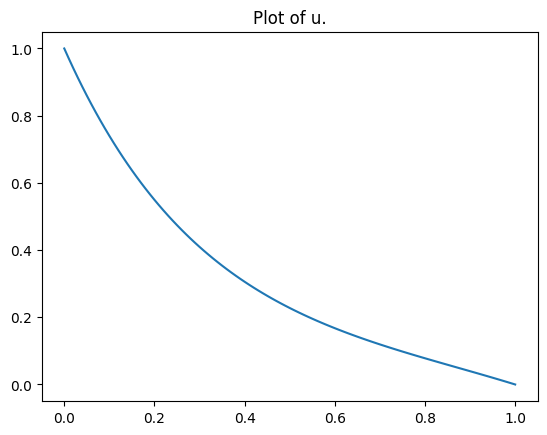
\includegraphics[width=0.5\linewidth]{Exercises/Chapter 2/Photos/7_graph.png}
        \caption{Depiction of the function found by using our modified finite element method. }
        \label{fig:problem_7}
    \end{figure}
\end{proof}

\begin{exer}
    For the BVP (2.3)–(2.4) on $D = (0, 1)$ with $p = 1, q = 0$, and constant $f$ , show that the Galerkin finite element matrix associated with polynomials of degree $r = 1$ is the tridiagonal matrix
    $$
    \begin{pmatrix}
        2/h & -1/h &  &  & \\
        -1/h & 2/h & -1/h & & \\
         &\ddots & \ddots & \ddots & \\
          & & \ddots & \ddots & -1/h\\
          & & & -1/h & 2/h
    \end{pmatrix}.
    $$
    Hence, determine that the finite element approximation is equivalent to a centred finite difference approximation.
\end{exer}
\begin{proof}
    This is very similar to Problem $6$. Notice that for each element we must compute 
    $\int_{e_k} \frac{d\phi_k(x)}{dx}^2 dx$ and  $\int_{e_k} \frac{d\phi_k(x)}{dx}^2 dx$. By translation invariance, we only need to compute 
    \begin{align*}
        \int_{e_k} \frac{d\phi_k(x)}{dx}^2 dx & = \int_0^h \frac{1}{h}^2 dx  = \frac{1}{h}\\
        \int_{e_k} \frac{d\phi_k(x)}{dx}\frac{d\phi_{k+1}}{dx} &= \int_0^h \frac{-1}{h}^2 dx  = \frac{-1}{h}.
    \end{align*}
    Adding these up give the tri-diagonal structure along the interior. Note we do not need to consider the end points as this problem has Dirichlet boundary conditions. I would like to use this to interpret finite difference methods as a special case of the more general finite element method. 
\end{proof}

\begin{exer}
    Algorithm 2.1 uses the Matlab backslash command to solve the piecewise linear Galerkin finite element system $Au = b$. By successively refining the mesh, investigate the efficiency of this solver for the linear systems associated with the BVP in Example 2.31, with respect to the dimension J
\end{exer}
\begin{proof}
    \tcr{Results are not clear. Sure I am making a mistake.}
\end{proof}
\begin{exer}
    By writing $e(x)\vert_{e_k}$ as a Fourier series $e(x)\vert_{e_k} = \sum_{n=1}^\infty a_n \sin\left(\frac{n\pi (x-z_{k-1})}{h}\right)$ in Theorem 2.32 as a Fourier sine series, show that 
    \begin{align*}
        \int_{z_{k-1}}^{z_k} e(x)^2 dx & = \frac{h}{2}\sum_{n=1}^\infty \abs{a_n}^2 \\
         \int_{z_{k-1}}^{z_k} e'(x)^2 dx & = \frac{h}{2}\sum_{n=1}^\infty \left(\frac{n\pi}{h}\right)^2\abs{a_n}^2 \\
          \int_{z_{k-1}}^{z_k} e''(x)^2 dx & = \frac{h}{2}\sum_{n=1}^\infty \left(\frac{n\pi}{h}\right)^4\abs{a_n}^2.
    \end{align*}
    and hence prove (2.43).
\end{exer}
\begin{proof}
    The existence of such a series follows from the fact that $u\in H^2(a,b) \cap H_0^1(a,b)$. As $u-I_h u \in H_0^1(a,b)\cap H^2(a,b)$, all sums that follow exist and are absolutely convergent so we do not need to worry about exchange of sums. 
    \par Given that such a series exists, we may explicitly compute 
    \begin{align*}
        \int_{z_{k-1}}^{z_k} e(x)^2 dx &= \sum_{n=1}^\infty \sum_{m=1}^\infty a_n a_m^* \int_{z_{k-1}}^{z_k} \sin\left(\frac{n\pi (x-z_{k-1})}{h}\right)\sin\left(\frac{m\pi (x-z_{k-1})}{h}\right) dx\\
        &=  \frac{1}{2}\sum_{n=1}^\infty \sum_{m=1}^\infty a_n a_m^* \int_{z_{k-1}}^{z_k} \cos\left(\frac{(n-m)\pi (x-z_{k-1})}{h}\right) - \cos\left(\frac{(n+m)\pi (x-z_{k-1})}{h}\right) dx.
    \end{align*}
    Thus it is sufficient to determine the behaviour of $$\int_{z_{k-1}}^{z_k} \cos\left(\frac{l\pi (x-z_{k-1})}{h}\right) dx, l\in \Z. $$ By direct computation if $l\neq 0$ we have
    \begin{align*}
        \int_{z_{k-1}}^{z_k} \cos\left(\frac{l\pi (x-z_{k-1})}{h}\right) dx = \left[\frac{h}{l\pi} \sin\left(\frac{l\pi (x-z_{k-1})}{h}\right)\right]_{z_{k-1}}^{z_k} = \frac{h}{l\pi} \left[\sin(l\pi) - \sin(0)\right] = 0. 
    \end{align*}
    If $l= 0$, of course we have the integral is $h$. Thus we have that 
     \begin{align*}
        \int_{z_{k-1}}^{z_k} e(x)^2 dx  &=  \frac{1}{2}\sum_{n=1}^\infty \sum_{m=1}^\infty a_n a_m^* h \delta_{m,n} \\
        &= \frac{h}{z}\sum_{n=1}^{\infty} \abs{a_n}^2.
    \end{align*}
    The others follow similarly by noting that the derivative multiplies each term in the sine series by $\frac{n\pi}{h}$ and using a similar orthogonality relation for cosine. 
\end{proof}

\begin{exer}
     Let $D = (0, 1)$ and define $e = u - I_h u$ as in Theorem 2.32.
    \begin{enumerate}[label=\alph*.]
        \item Use Exercise 1.14(a) and apply a change of variables to show that 
        $$\int_0^h e(y)^2 dy \leq h^2 \int_0^h  e'(y)^2 dy.$$
        \item Similarly, show that 
        $$\int_0^h e'(y)^2 dy \leq h^2 \int_0^h e''(y)^2 dy.$$
        \item  Hence, prove Theorem 2.32 without using Exercise 2.10. Compare the constant K in your error bound with the one in (2.44).
    \end{enumerate}
\end{exer}
\begin{proof}
    Note that $e\in H_0^1(0,1)$. Note that $e(x/h) \in H_0^1(0,1/h)$ by essentially chain rule or change of variables. Thus we may apply 
    \begin{enumerate}
        \item \tcr{Still to Prove}
        \item \tcr{Still to Prove}
        \item \tcr{Still to Prove}
    \end{enumerate}
\end{proof}

\begin{exer}
    Modify Algorithm 2.1 and compute the piecewise linear finite element approximation to the solution of the BVP (2.3)–(2.4) with data chosen as in Example 2.5. Compare the approximation with the exact solution at the vertices of the mesh. What do you observe?
\end{exer}
\begin{proof}
    \tcr{Code it all up. Just need to implement the forcing function} 
\end{proof}

\begin{exer}
    \begin{enumerate}[label=\alph*.]
        \item Let $z_k \in [0,1]$ and find the Green's function satisfying 
        $$-\frac{\partial^2 G(x,z_k)}{\partial x^2 } = \delta(x-z_k)$$
        and boundary conditions $G(0,z_k) = G(1,z_k) = 0.$
        \item Let $z_k$ be any vertex of the mesh associated with a piece-wise linear finite element discretization of the BVP in Example 2.5. Use your answer to part (a) to explain your observations in Exercise 2.12.
    \end{enumerate}
\end{exer}
\begin{proof}
    \begin{enumerate}[label=\alph*.]
        \item This answer was actually provided in the text of Chapter 1. The answer is 
        $$G(x,z_k) = \begin{cases}
            x(1-z_k)& x \leq z_k \\
            z_k(1-x)& x > z_k 
        \end{cases}.$$
        \item \tcr{Compare after completing 12. Notice that this is very similar to a linear finite element mesh.}
\end{enumerate}
\end{proof}
\begin{exer}
    Let Assumption 2.34 hold. Use the Lax–Milgram Lemma to prove the existence and uniqueness of $u_0 \in V$ satisfying (2.58) and hence prove Theorem 2.42.
\end{exer}
\begin{proof}
    Under assumption 2.34, the the energy norm induces an inner product on $H_0^1.$ It is also clearly coercive, with an easy lower bound given by $p_0/(1+K)$ where $K$ is the Poincar\'e constant of the domain. It is also bounded as $p,q$ are bounded. $\ell$ is also clearly linear, and bounded by Cauchy-Schwartz. Thus by Lax-Milgram there exists a unique solution.
\end{proof}

\begin{exer}
    Solve (2.89) in \cite{lord2014introduction} and hence find the local piece wise linear finite element basis functions $\phi_1^k, \phi_2^k, \phi_3^k$ for an element $\Delta_k$ in two dimensions. Similarly, find the six piecewise quadratic basis functions $\phi_k^i, i = 1,...,6$ associated with r =2 .
\end{exer}
\begin{proof}
    (2.89) in \cite{lord2014introduction} is written as 
    $$\begin{pmatrix}
        x_1^k & y_1^k & 1 \\
        x_2^k & y_2^k & 1 \\
        x_3^k & y_3^k & 1
    \end{pmatrix}\begin{pmatrix}
        a_i\\
        b_i\\
        c_i
    \end{pmatrix} = \mathbf{e}_i.$$
    This can be found explicitly by finding the inverse of this matrix. We solve this explicitly using Cramer's rule. 
    \begin{gather*}
        \text{det}A = x_1^k\left(y_2^k - y_3^k\right)-y_1^k\left(x_2^k-x_3^k\right)+\left(x_2^k y_3^k - x_3^k y_2^k\right) = \mathbf{x}\times \mathbf{y}\cdot \mathbf{1}\\
        a_i = \frac{\mathbf{\mathbf{e}_i \times \mathbf{y}\cdot \mathbf{1}}}{\mathbf{x}\times \mathbf{y}\cdot \mathbf{1}} = \frac{\mathbf{\mathbf{y}\times \mathbf{1}} \cdot \mathbf{e}_i}{\mathbf{x}\times \mathbf{y}\cdot \mathbf{1}}\\
        b_i = \frac{\mathbf{\mathbf{x} \times \mathbf{e}_i\cdot \mathbf{1}}}{\mathbf{x}\times \mathbf{y}\cdot \mathbf{1}} = \frac{\mathbf{\mathbf{1}\times \mathbf{x}} \cdot \mathbf{e}_i}{\mathbf{x}\times \mathbf{y}\cdot \mathbf{1}}\\
        c_i = \frac{\mathbf{\mathbf{x} \times \mathbf{y}\cdot \mathbf{e}_i}}{\mathbf{x}\times \mathbf{y}\cdot \mathbf{1}} 
    \end{gather*}
    \par For the quadratic polynomials, we could set up a similar system of equations. However, notice it is sufficient to find six independent polynomials which vanish in the appropriate frame. We will see this is much easier in the standard frame, so for now we will simply note that the mapping can be found in the refernce frame and then translated back by noting
    $$\begin{bmatrix}
        x\\y
    \end{bmatrix}=\begin{bmatrix}
        x_2^k-x_1^k & x_3^k-x_1^k\\
        y_2^k -y_1^k & y_3^k-y_3^k
    \end{bmatrix}\begin{bmatrix}
        t\\s
    \end{bmatrix}+\begin{bmatrix}
        x_1^k\\y_1^k
    \end{bmatrix}.$$
    As this mapping is affine, it clearly won't change the polynomial degree.
\end{proof}

\begin{exer}
    Show that the local piecewise linear basis functions $\psi_1, \psi_2,\psi_3$ associated with the reference element $\Delta_*$ in Figure 2.15 are given by (2.91) in \cite{lord2014introduction}. Similarly, find the six quadratic reference element basis functions associated with r =2. 
\end{exer}
\begin{proof}
    We can apply the previous theorem using $\mathbf{x} = \begin{bmatrix}
        0 & 1 & 0
    \end{bmatrix}, \mathbf{y} = \begin{bmatrix}
        0 & 0 & 1
    \end{bmatrix}.$
    The determinant is then clearly $1$ and 
    \begin{align*}
        a_i &= \delta_{i,2}-\delta_{i,1}\\
        b_i &= \delta_{i,3}-\delta_{i,1}\\
        c_i &= \delta_{i,1}
    \end{align*}
    Applying the definition of $a,b,c$ gives the required results. 
    \par For the quadratic case, we first focus on the elements based at $(1/2,0),(1/2,1/2),(0,1/2)$. Note these are the essentially only new members. Also, the previous polynomials vanish not just at their assigned points but along the whole line. This we may take their products to get teh required elements:
    \begin{gather*}
        \psi_4(s,t) = ct(1-t-s), \phi_4(1/2,0)=1\implies  \psi_4(s,t) = 4t(1-t-s)\\
        \psi_5(s,t) = cts, \phi_5(1/2,1/2)=1\implies  \psi_5(s,t) = 4ts\\
        \psi_6(s,t) = cs(1-t-s), \phi_6(0,1/2)=1\implies  \psi_6(s,t) = 4s(1-t-s)
    \end{gather*}
    It then suffices to subtract off these values from our original polynomials to obtain the new ones.
     \begin{align*}
        \psi_1(s,t) &= t-1/2\psi_4-1/2\psi_5 = t-2t(1-t-s)-2ts=2t^2-t\\
        \psi_2(s,t) &= 1-t-s- 1/2\psi_4-1/2\psi_6=1-t-s-2t(1-t-s)-2s(1-t-s)\\
        &=(1-2t-2s)(1-t-s)\\
        \psi_6(s,t) &= s-1/2\psi_6-1/2\psi_5=s-2s(1-t-s)-2ts=2s^2-s\\
    \end{align*}
\end{proof}

\begin{exer}
    Show that the mapping (2.92)–(2.93) in \cite{lord2014introduction} is affine and show that, for the triangle $\Delta_k$ with vertices $(h,h)$,$(2h,h)$ and $(h,2h)$, the mapping corresponds to a certain shift and scaling of the reference element.
\end{exer}
\begin{proof}
    A mapping is affine if and only if it can be written in the form $Ax+b$ where $A$ is a linear operator. In this case 
    \begin{gather}
        \begin{bmatrix}
            x\\y
        \end{bmatrix}=\begin{bmatrix}
            x_2^k-x_1^k & x_3^k-x_1^k\\
            y_2^k-y_1^k & y_3^k-y_1^k
        \end{bmatrix}\begin{bmatrix}
            s\\t
        \end{bmatrix}+\begin{bmatrix}
            x_1^k\\y_1^k
        \end{bmatrix}.
    \end{gather}
    Thus the mapping is affine. In the special case mentioned:
    \begin{gather}
        \begin{bmatrix}
            x\\y
        \end{bmatrix}=\begin{bmatrix}
            h & 0\\
            0 & h
        \end{bmatrix}\begin{bmatrix}
            s\\t
        \end{bmatrix}+\begin{bmatrix}
            h\\h
        \end{bmatrix} = h\left(\begin{bmatrix}
            s\\t
        \end{bmatrix}+\begin{bmatrix}
            1\\1
        \end{bmatrix}\right).
    \end{gather}
    Thus it is exactly a shift plus a scale by $h$.
\end{proof}

\begin{exer}
Let $r=1$ and assume the diffusion coefficient $a$ and the function $f$ are point-wise constant on the elements of the mesh.
\begin{enumerate}[label=\alph*.]
    \item Derive the element matrix and the element vector for the general triangle $\Delta_k$ with vertices $(x_1^k,y_1^k),(x_2^k,y_2^k),(x_3^k,y_3^k).$
    \item Now fix $D=(0,1)^2$ and assume the mesh is generated using Algorithm 2.4 in \cite{lord2014introduction}. Show that
    $$A^k=a_k A^*, b_k= h^2 f_k b^*, \ \forall \ \Delta_k \in \mathcal{T}_h.$$
    where $a_k$ and $f_k$ are the values in $\Delta_k$ and 
    \begin{align*}
        A^* =\begin{pmatrix}
            1 & -1/2 & -1/2\\
            -1/2 & 1/2 & 0\\
            -1/2 & 0 &1/2
        \end{pmatrix} && b^* = \begin{bmatrix}
            1/6\\1/6\\1/6
        \end{bmatrix}.
    \end{align*}
\end{enumerate}
    
\end{exer}
\begin{proof}
\begin{enumerate}[label=\alph*.]
    \item \tcr{I think this is annoying and not the correct order to do this problem in.}
    \item Let us assume we are looking at the reference element scaled by $1/h$. Note every element generated by 2.4 is of this type with a translation and reflection which will not change any of the integrals. We must thus compute  the following integrals
    \begin{align*}
        \int_0^h \int_0^t a_k \begin{bmatrix}
            -1/h\\-1/h
        \end{bmatrix}\cdot\begin{bmatrix}
            -1/h\\-1/h
        \end{bmatrix} ds dt = \frac{2a_k}{h^2}\frac{h^2}{2}=a_k\\
        \int_0^h \int_0^t a_k \begin{bmatrix}
            -1/h\\-1/h
        \end{bmatrix}\cdot\begin{bmatrix}
            1/h\\0
        \end{bmatrix} ds dt = \frac{-a_k}{h^2}\frac{h^2}{2}=\frac{-a_k}{2}\\
        \int_0^h \int_0^t a_k \begin{bmatrix}
            -1/h\\-1/h
        \end{bmatrix}\cdot\begin{bmatrix}
            0\\1/h
        \end{bmatrix} ds dt = \frac{-a_k}{h^2}\frac{h^2}{2}=\frac{-a_k}{2}\\
        \int_0^h \int_0^t a_k \begin{bmatrix}
            1/h\\0
        \end{bmatrix}\cdot\begin{bmatrix}
            1/h\\0
        \end{bmatrix} ds dt = \frac{a_k}{h^2}\frac{h^2}{2}=\frac{a_k}{2}\\
        \int_0^h \int_0^t a_k \begin{bmatrix}
            1/h\\0
        \end{bmatrix}\cdot\begin{bmatrix}
            0\\1/h
        \end{bmatrix} ds dt = 0\\
        \int_0^h \int_0^t a_k \begin{bmatrix}
            0\\1/h
        \end{bmatrix}\cdot\begin{bmatrix}
            0\\1/h
        \end{bmatrix} ds dt = \frac{a_k}{h^2}\frac{h^2}{2}=\frac{a_k}{2}.
    \end{align*}
\end{enumerate}
Which gives all of the coefficients as desired. For $b$, we simply need to compute
\begin{align*}
    \int_0^h\int_0^t f_k \frac{s}{h} ds dt &= \int_0^h \frac{f_k t^2}{2h}dt = \frac{f_k h^2}{6}\\
    \int_0^h\int_0^s f_k \frac{t}{h} dt ds &= \int_0^h \frac{f_k s^2}{2h}ds = \frac{f_k h^2}{6}\\
    \int_0^h\int_0^t f_k \left(1-\frac{s}{h}-\frac{t}{h}\right) ds dt &= f_k \int_0^h t -\frac{t^2}{2h}-\frac{t^2}{h}dt = f_k \int_0^h t -\frac{t^2}{2h}-\frac{t^2}{h}dt \\
    &= \frac{f_k h^2}{2}-\frac{f_k h^2}{6}-\frac{f_k h^2}{3}=\frac{f_k h^2}{6}.
\end{align*}
    Exactly as desired.
\end{proof}

\begin{exer}
    Use Algorithms 2.4 and 2.7 to generate the Galerkin finite element schemes associated with the BVP in Example 2.63 (for both choices of $a$) on successively refined meshes.
    \begin{enumerate}[label=\alph*.]
        \item Investigate the efficiency of the solve function with respect to $J$.
        \item Solve the system using the conjugate gradient solver. Record the number of iterations required. What do you observe?
    \end{enumerate}
\end{exer}
\begin{proof}
    
\end{proof}

\printbibliography
\end{document}